\documentclass[12pt]{article}
\usepackage[spanish]{babel}
\usepackage[utf8]{inputenc}
\usepackage{amsmath}
\usepackage{listings}
\usepackage[usenames]{color}
\definecolor{gray97}{gray}{.97}
\definecolor{gray75}{gray}{.75}
\definecolor{gray45}{gray}{.45}
\definecolor{azul1}{RGB}{141,198,163}
\definecolor{azul2}{RGB}{24,107,122}
\definecolor{verde1}{RGB}{44,186,34}

\usepackage{textcomp}
\lstset{
		frame=Ltb,
		framerule=1pt,
		framextopmargin=3pt,
		framexbottommargin=3pt,
		framexleftmargin=0.4cm,
		framesep=0pt,
		rulesep=.4pt,
		backgroundcolor=\color{gray97},
		rulesepcolor=,
        tabsize=4,
        rulecolor=\color{azul1},
        basicstyle=\scriptsize\rmfamily,
        upquote=true,
        aboveskip={1.5\baselineskip},
        columns=fixed,
        showstringspaces=false,
        extendedchars=true,
        breaklines=true,
        prebreak = \raisebox{0ex}[0ex][0ex]{\ensuremath{\hookleftarrow}},
        showtabs=false,
        showspaces=false,
        showstringspaces=false,
        identifierstyle=\rmfamily,
        keywordstyle=\color[rgb]{0,0,1},
        commentstyle=\color[rgb]{0.133,0.545,0.133},
        stringstyle=\color[rgb]{0.627,0.126,0.941},
        keywordstyle=\bfseries,
        %
		numbers=left,
		numbersep=15pt,
		numberstyle=\tiny,
		numberfirstline = false,
		breaklines=true,
		}
\usepackage{graphicx}
\usepackage[colorinlistoftodos]{todonotes}
\usepackage{natbib} %citas bibliograficas estilo APA :p
\usepackage{eso-pic}
\usepackage{avant}
\usepackage[top=2cm,bottom=2cm,left=2.5cm,right=3cm,headsep=8pt,a4paper]{geometry}
\usepackage{fancyhdr}
\pagestyle{fancy}
\fancyhf{}
%\fancyhead[LE,RO]{}
\fancyhead[RE,LO]{Procesamiento de Señales II}
\fancyfoot[CE,CO]{\leftmark}
\fancyfoot[LE,RO]{\thepage}
\renewcommand{\headrulewidth}{2pt}
\renewcommand{\footrulewidth}{1pt}
\usepackage{tabu}
\usepackage{array}
\usepackage{multirow}
\usepackage{amssymb}
\usepackage{makeidx}
\graphicspath{ {images/} }
\usepackage{wrapfig}
\usepackage{enumerate}
\usepackage{amsmath,tikz}
\usetikzlibrary{matrix}
\usepackage{steinmetz}
\newcommand*{\horzbar}{\rule[0.05ex]{2.5ex}{0.5pt}}
\usepackage{calc}
\date{\today}


\begin{document}

\begin{titlepage}
\newcommand{\HRule}{\rule{\linewidth}{0.5mm}} 
\center
\textsc{\LARGE  Benemérita Universidad \\[0.2cm] Autónoma de Puebla}\\[1.5cm] 

\includegraphics[width=4cm]{escudo.jpg}\\[1cm]
\textsc{\Large Facultad de Ciencias de la Electrónica}\\[0.5cm] 
\textsc{\large Licenciatura en Electrónica}\\[0.5cm]
\HRule \\[0.4cm]
{ \huge \bfseries Reporte de práctica 1: Generación de señales con DSP.}\\[0.4cm] 
\HRule \\[1.5cm]
\begin{minipage}{\textwidth}
\center 

\emph{Profesor:} \\
Fernando López Marcos \\[1cm]

\begin{tabular}{ll}
\emph{Alumnos:} & \emph{Número de Matrícula:}\\
Hanan Ronaldo Quispe Condori  & 555010653 \\
Erick Sandro Niño García & 201631150\\
Carlos Alfredo Vega Aguilar & 201632131 \\
\end{tabular}
\end{minipage}\\[2cm]
\today
\end{titlepage}

%\newpage
%~\vfill
%\thispagestyle{empty}
%\begin{figure}[hbtp]


%\includegraphics[width=4cm]{IMAGENES/motordc}
%\end{figure}
%\noindent \textsc{Trabajo Encargado: Problemas en MatLab \\ Máquinas Eléctricas \\ Universidad Nacional de San Antonio abad del Cusco}\\
%noindent \textsc{Ingeniería Electrónica }\\
%\noindent \textit{Tercera revisión, \today}

%\tableofcontents indice bloqueado xD

\newpage

\section{Introducción}

Un procesador digital de señales o DSP  es un sistema que tiene un conjunto de instrucciones,
 hardware y software optimizados para aplicaciones  a muy alta velocidad. Es especialmente útil para el procesado y 
representación de señales analógicas en tiempo real. Pueden
realizar operaciones matemáticas complejas en un solo ciclo de reloj.La diferencia principal entre un DSP y
un microprocesador es que
el DSP es muy rápido para un tipo de operaciones concretas, ya que tiene instrucciones especiales para ellas, y las puede
realizar de forma paralela.
\\\\
Un ejemplo puede ser que un microprocesador  necesita 5
ciclos de reloj para una suma y 32 ciclos
de reloj para una multiplicación, sin embargo un DSP puede realizar una operación MAC (Multiply, Add, y
Accumulate) es decir permite multiplicar, sumar y guardar el resultado en un solo
ciclo de reloj.
\\
\\
Este reporte contiene todo lo relacionado con la primera práctica de la asignatura, desarrollada por el equipo conformado por los estudiantes mencionados en la portada del presente documento.
\\
\\
La práctica en términos generales consiste en tener el primer acercamiento con la tarjeta de desarrollo C6713 usándola para generar sintéticamente un tono. Con la ayuda de MATLAB para realizar el muestreo de un fragmento de un archivo de audio que contiene el sonido de un saxofón, las líneas de código de un programa en lenguaje C proporcionadas por el profesor y el uso del software Code Composer Studio para cargar el programa a la tarjeta, se buscará cumplir con los objetivos de esta primera práctica.
\\
\\
Cabe mencionar que, se eligió una versión específica del software Code Composer (7.1) para evitar problemas de compatibilidad con la tarjeta. Además, acto seguido de la instalación, se siguió un tutorial que el profesor nos mencionó para tener un primer acercamiento con el software, instalar complementos necesarios para poder programar la tarjeta y tener listo un programa de prueba (Blynk) para cargarlo en laboratorio al C6713.

\section{Objetivos}
Saber qué es un DSP.\\\\
Familiarizarse con la tarjeta de desarrollo C6713 mediante la replicación de una señal adquirida de forma externa.
\\\\
Conseguir que el tono sintético sea semejante al tono original.

\section{Desarrollo}
El archivo de audio usado está en formato .wav, este formato admite diversas resoluciones y velocidades de muestreo por lo cual se revisó que la frecuencia de muestreo de dicho archivo sea de 44100 Hz como se especificó en la guía proporcionada, se utilizó la herramienta $mediainfo$ para esta revisión.

\begin{figure}[h]
    \centering
        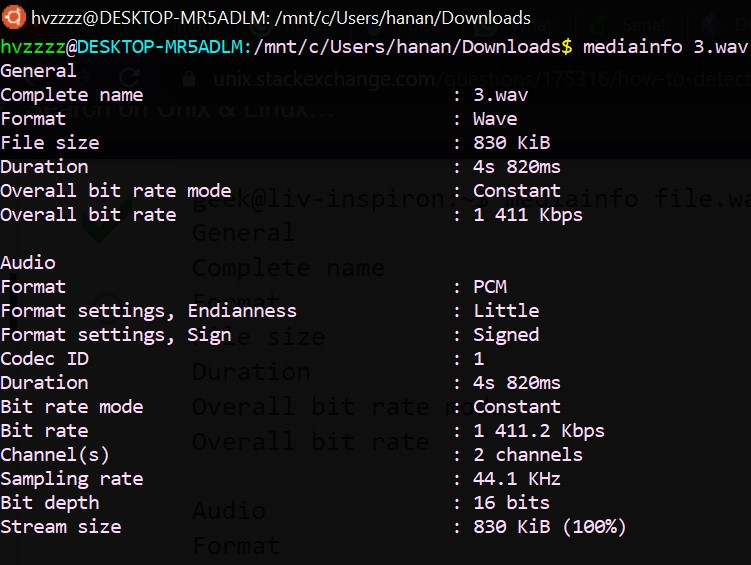
\includegraphics[width=6cm,height=5cm]{samp_freq.jpg}
        \caption{Información del Archivo de Audio.}
\end{figure}

Matlab fue el software empleado para la extracción de las muestras de un periodo de la señal, con este fin se procedió a importar el archivo de audio mediante el siguiente script.

\lstinputlisting[language=Matlab]{audio_extract_ini.m}

En este script se usó la función $audioread$ que nos permite hacer la extracción.

La gráfica de las muestras es la siguiente.

%\vspace{20mm}

\begin{figure}[h]
    \centering
        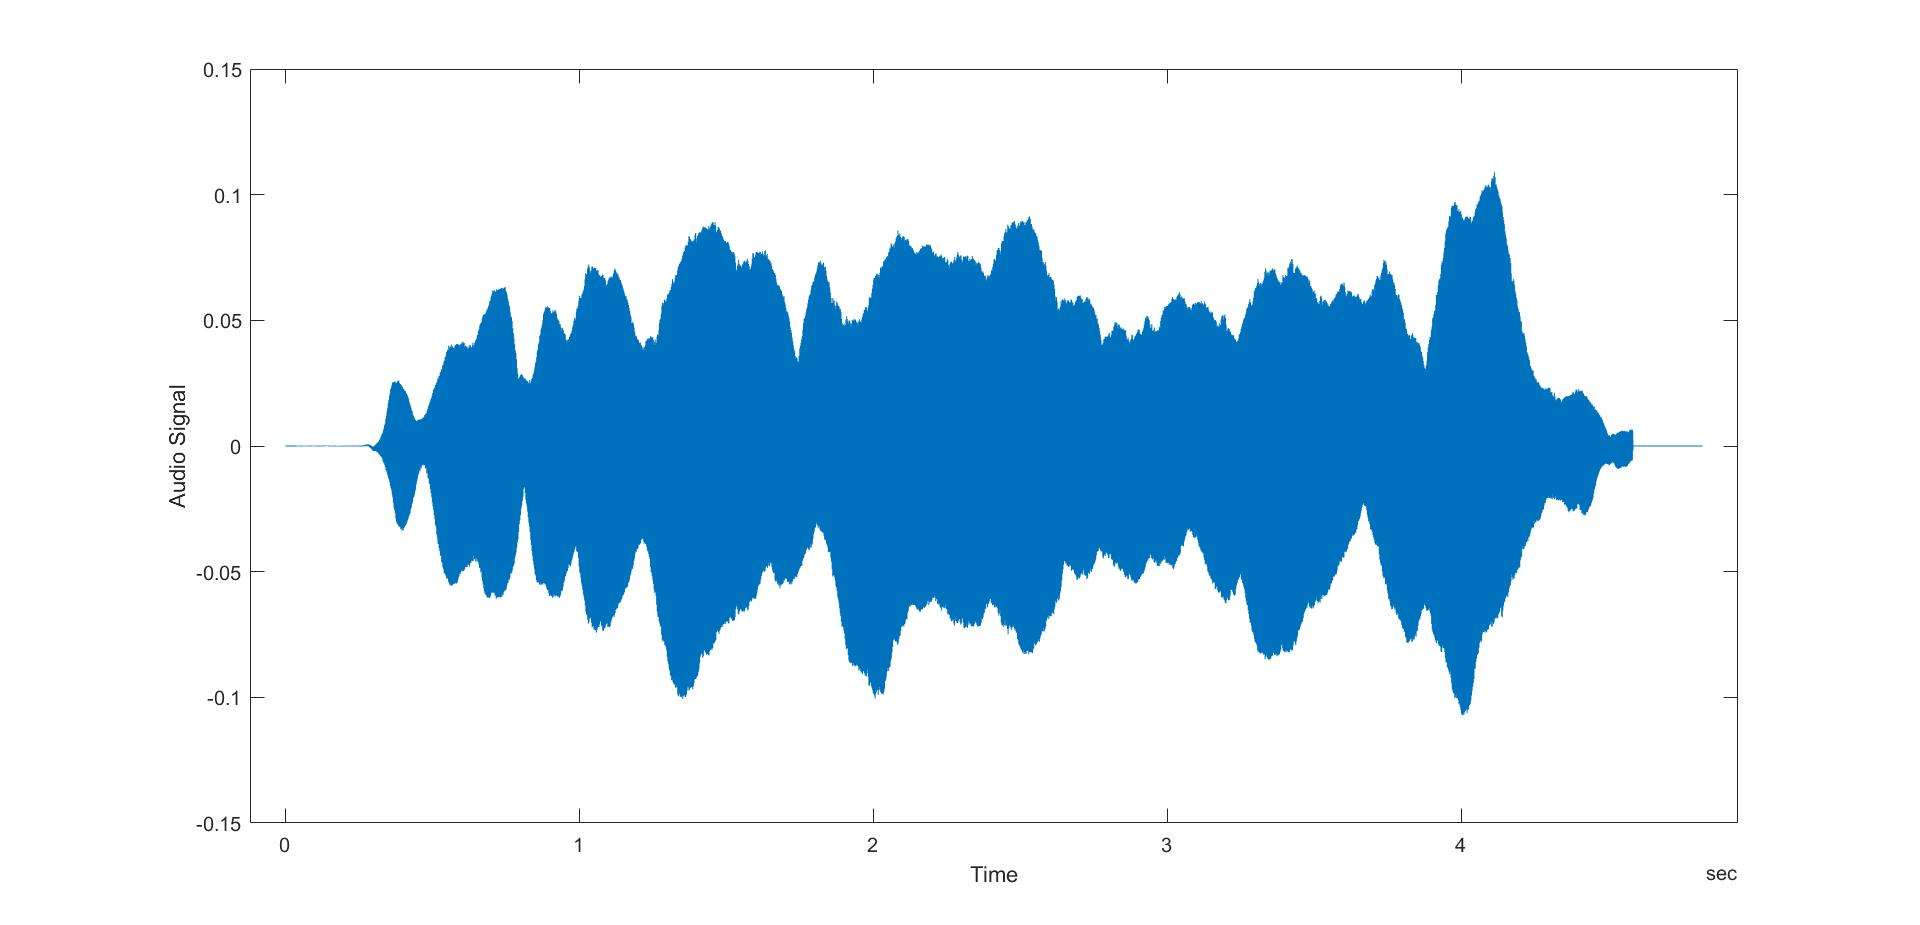
\includegraphics[width=15cm,height=5cm]{audiocompleto.jpg}
        \caption{Audio Completo.}
\end{figure}

Estas muestras corresponden al sonido producido por un saxofón alto. A simple vista no se puede apreciar su periodicidad pero, al hacer zoom a la imágen se podrá ir apreciando tal y como se muestra en las siguientes figuras.

\begin{figure}[h]
    \centering
        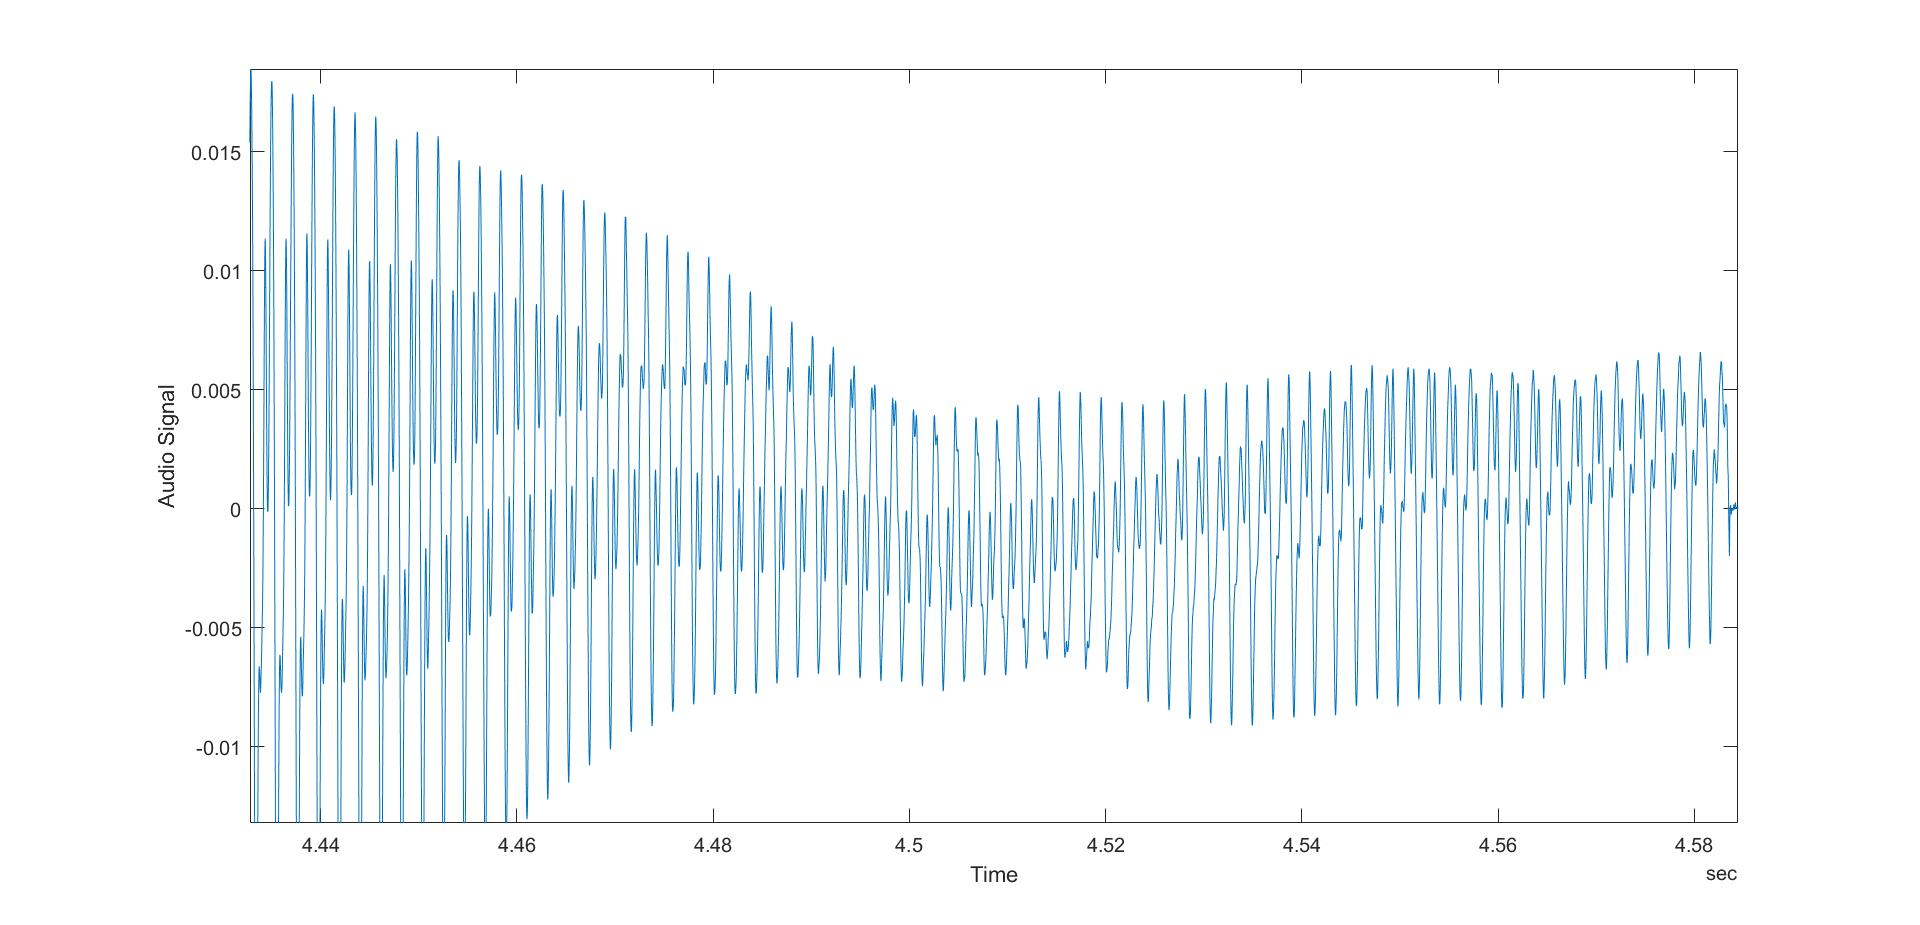
\includegraphics[width=8cm,height=5cm]{untitled.jpg}
        \caption{Parte del audio.}
\end{figure}

De la figura 3 solo necesitamos extraer las muestras de un periodo de la señal, se pudo escoger cualquier periodo, para esta práctica se eligieron las muestras entre los puntos que se muestran en la siguiente figura.

\vspace{19mm}
\begin{figure}[h]
    \centering
        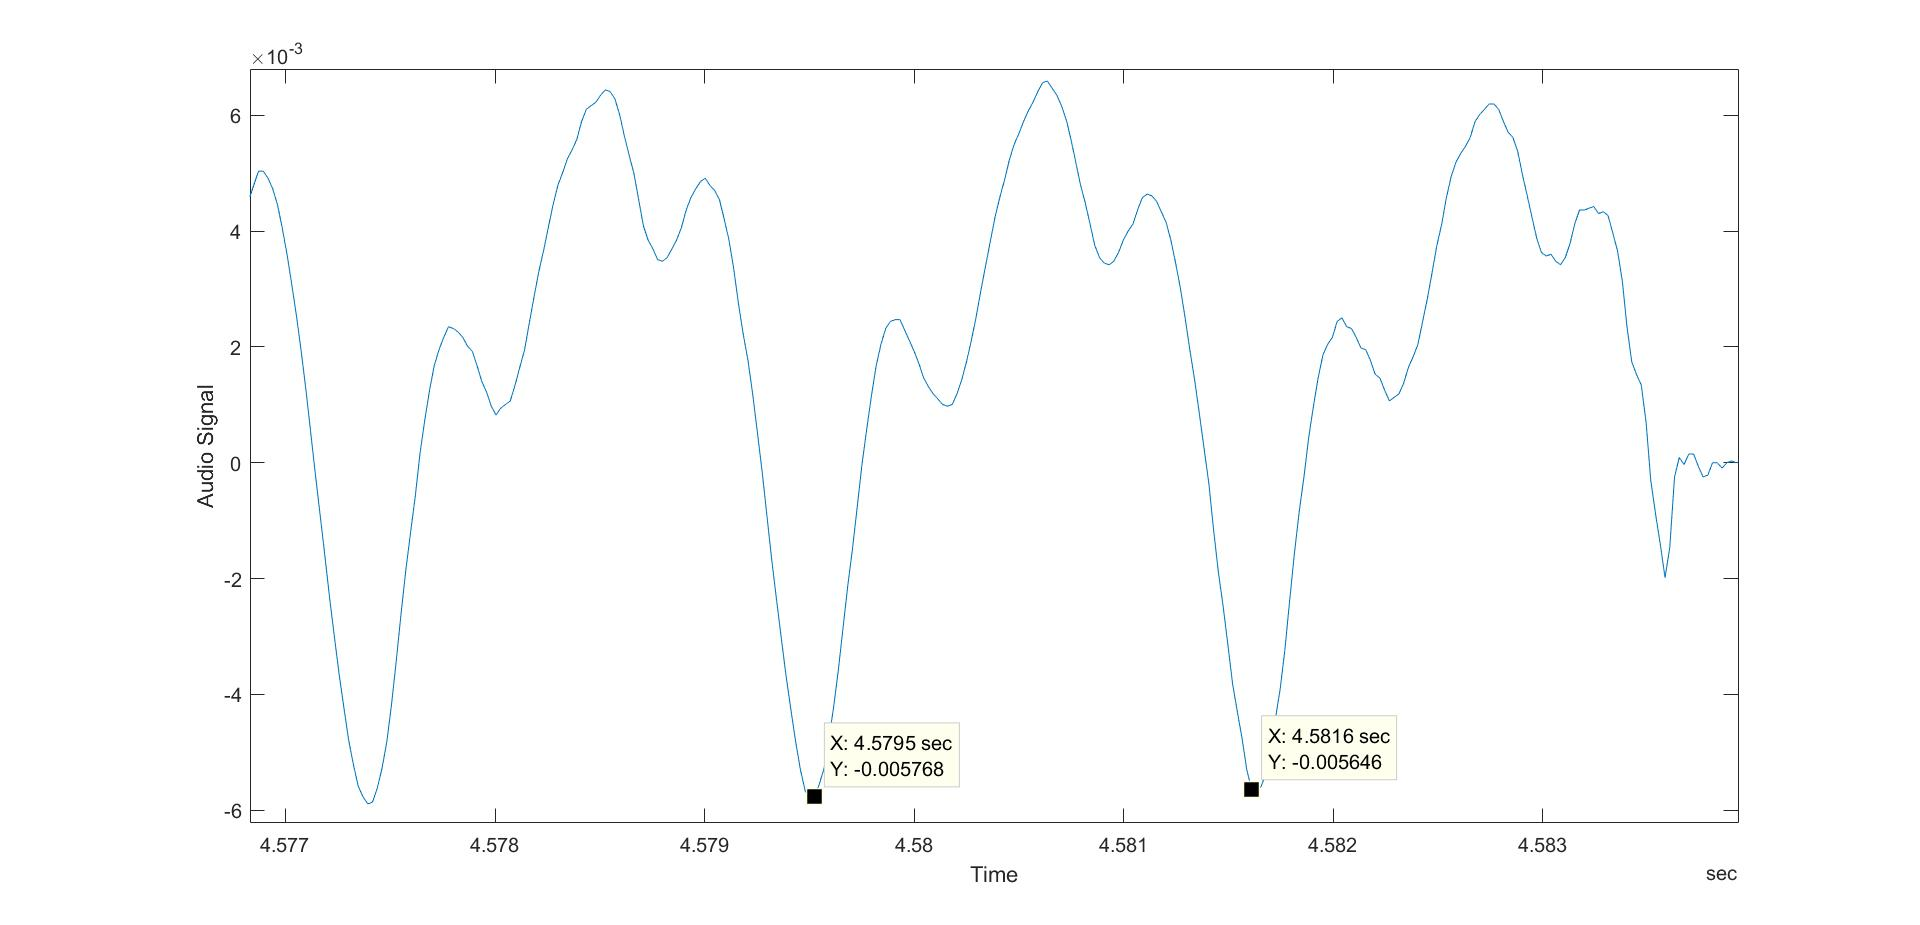
\includegraphics[width=15cm,height=5cm]{tamano_vector.jpg}
        \caption{Periodo Elegido.}
\end{figure}

Las muestras se extrajeron mediante el siguiente script.
\\
\\
%\vspace{20mm}
\lstinputlisting[language=Matlab]{audio_extract_muestras.m}

Se extrajo un subvector almacenado con el nombre de $muestras\_periodo$ con las posiciones correspondientes al periodo elegido.

Al graficar estas muestras se obtuvo la siguiente gráfica.

\begin{figure}[h]
    \centering
        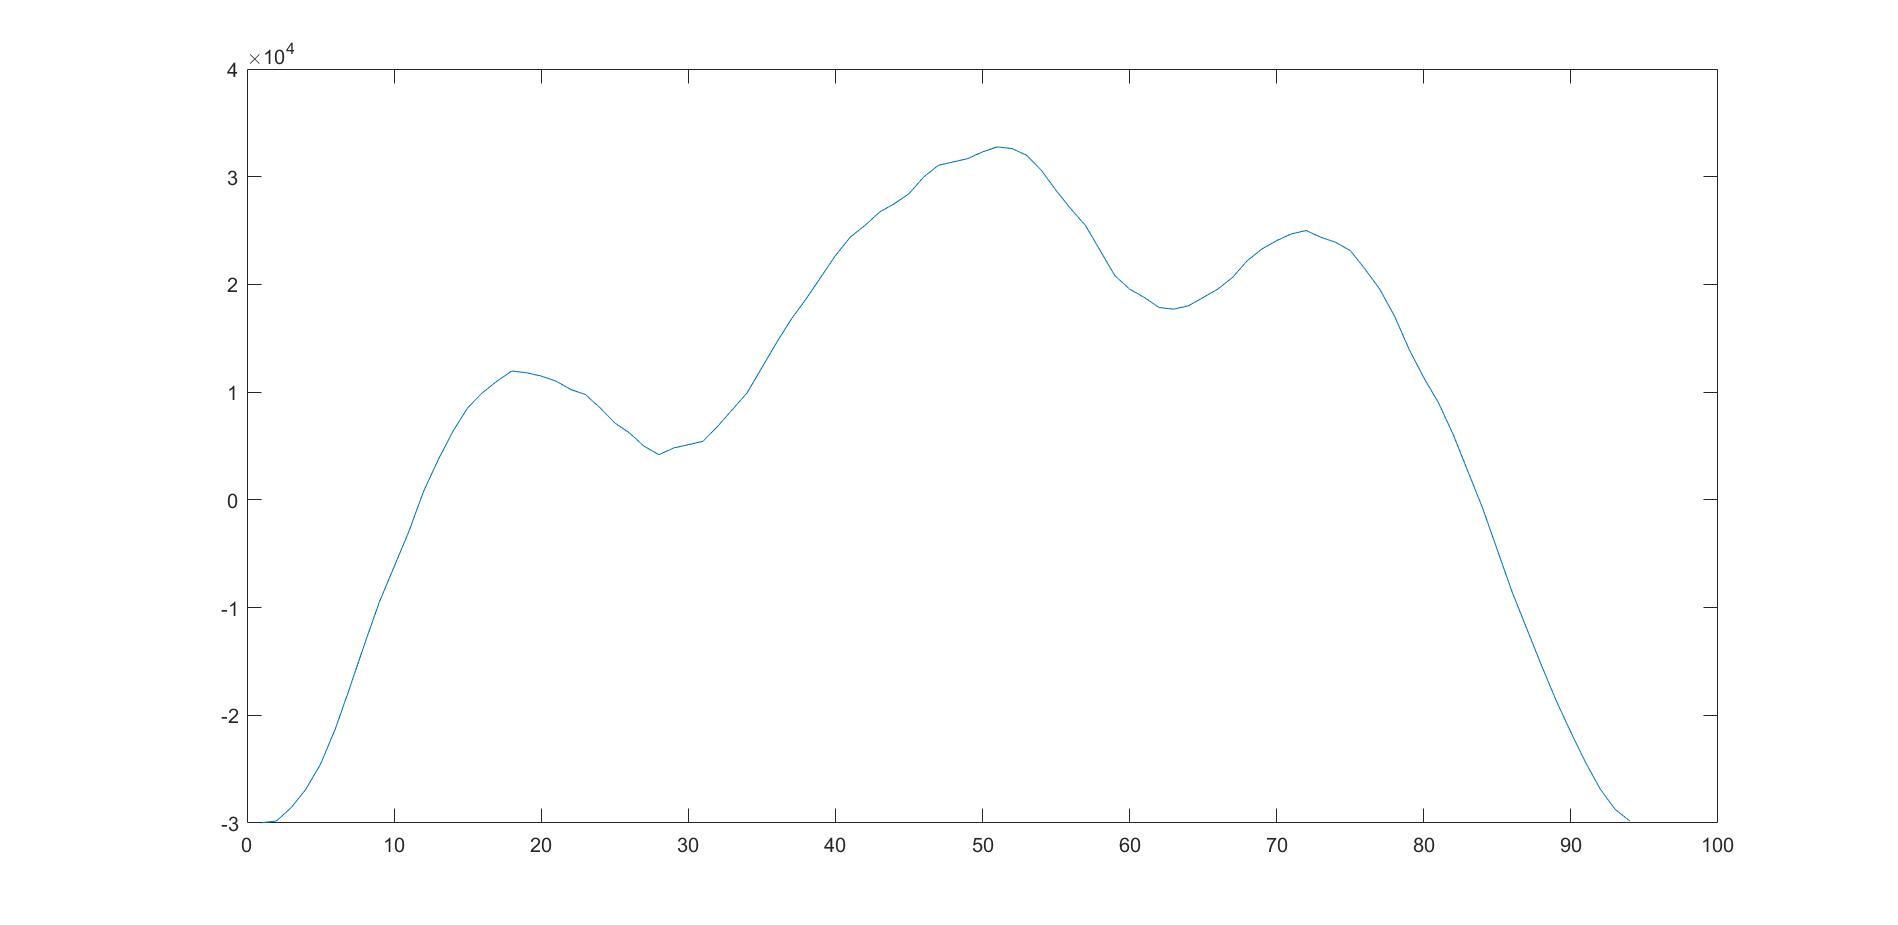
\includegraphics[width=15cm,height=7cm]{muestras.jpg}
        \caption{Muestras.}
\end{figure}

Despues se tuvieron que escalar estos valores al rango de $\lbrack-32768,32768 \rbrack$ para poder ser usados en el DSP ya que este posee una resolución de 16 bits, para esto, se extrajo el valor máximo del vector y por regla de 3 simple, se calculó un factor de escalamiento que se guardo en la variable $factor$ seguidamente se multiplicó al vector $muestras\_periodo$ por este factor de escalamiento y se redondearon sus valores. Como resultado de este proceso se obtuvieron 94 muestras, estas se usarán para reconstruir sintecticamente la señal original.

El profesor nos proporcionó el código a usar en el DSP, restando al equipo modificar el vector que estaba en el código colocando el vector que nosotros obtuvimos resultado del muestreo en Matlab.

\lstinputlisting[language=C++]{changes.cpp}

Llegados a este punto, todo está listo para cargar el programa a la tarjeta mediante Code Composer.


\begin{figure}[h]
    \centering
        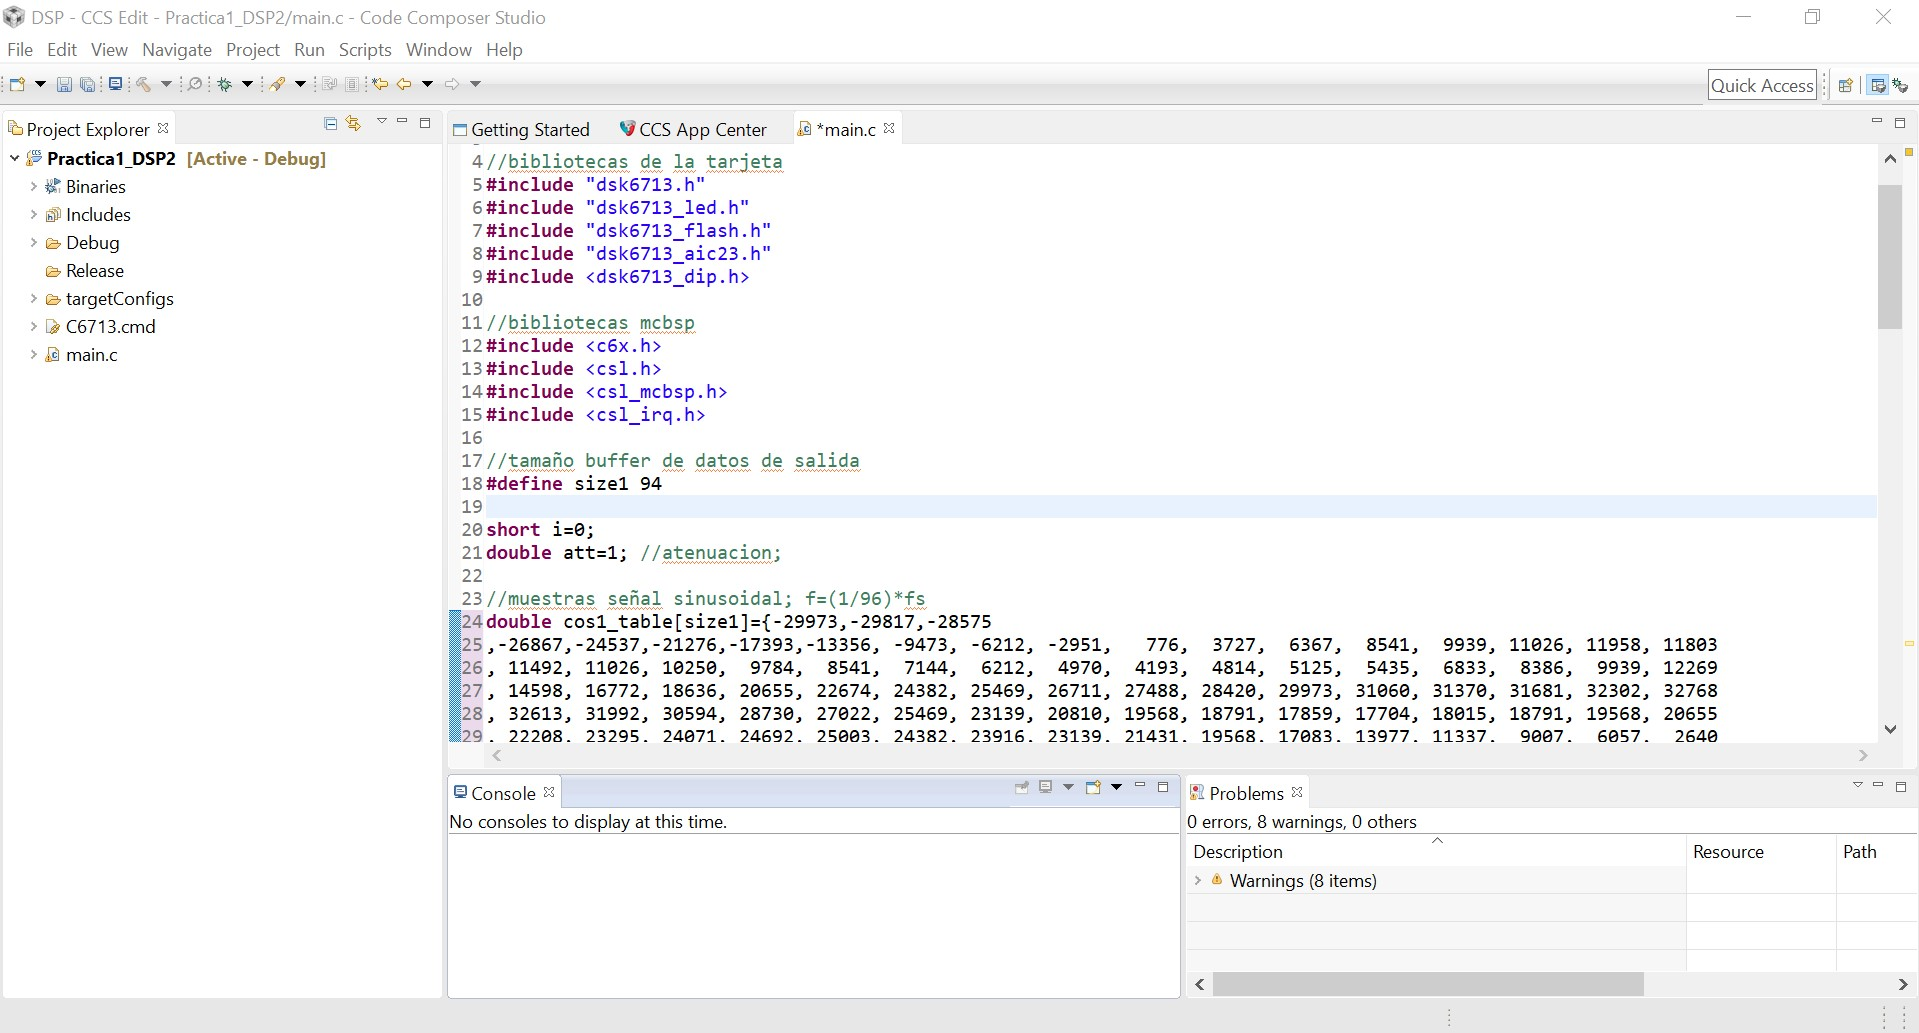
\includegraphics[width=15cm,height=8cm]{code_composer.jpg}
        \caption{Entorno Code Composer.}
\end{figure}

%\vspace{70mm}
\begin{figure}[h]
    \centering
        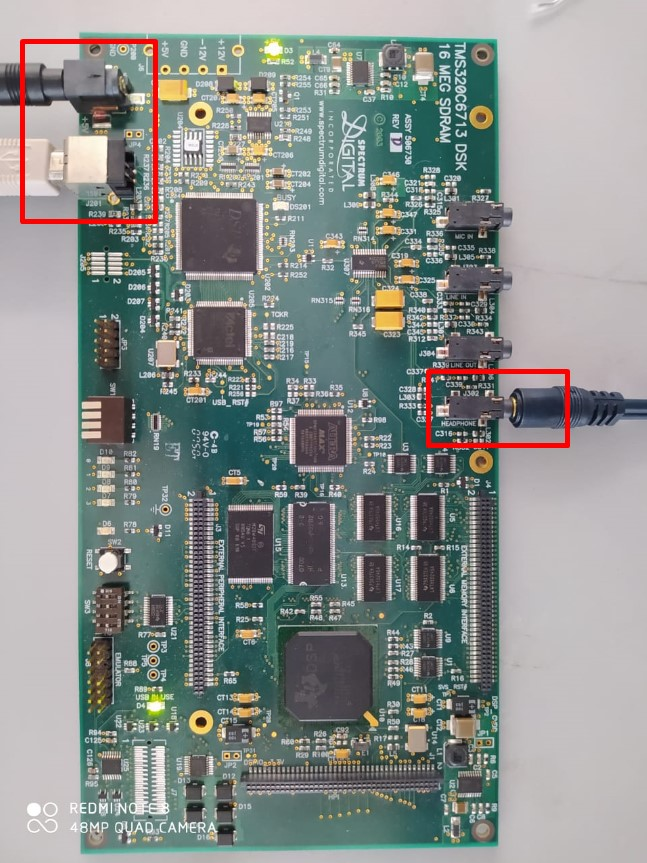
\includegraphics[width=7cm,height=6cm]{tarjeta.jpg}
        \caption{DSP.}
\end{figure}

En la tarjeta se hicieron las siguientes conexiones: en la salida de audio se conectó un cable de jack 3.5mm a RCA con adaptadores a BNC para ver la forma de onda de salida en el osciloscopio, las otras conexiones son de alimentación de la tarjeta y comunicación con PC. 

\section{Resultados}
Se muestra a continuación una fotografía de la señal generada por la tarjeta después de haberle cargado el programa creado.
%\vspace{30mm}
\begin{figure}[h]
\centering
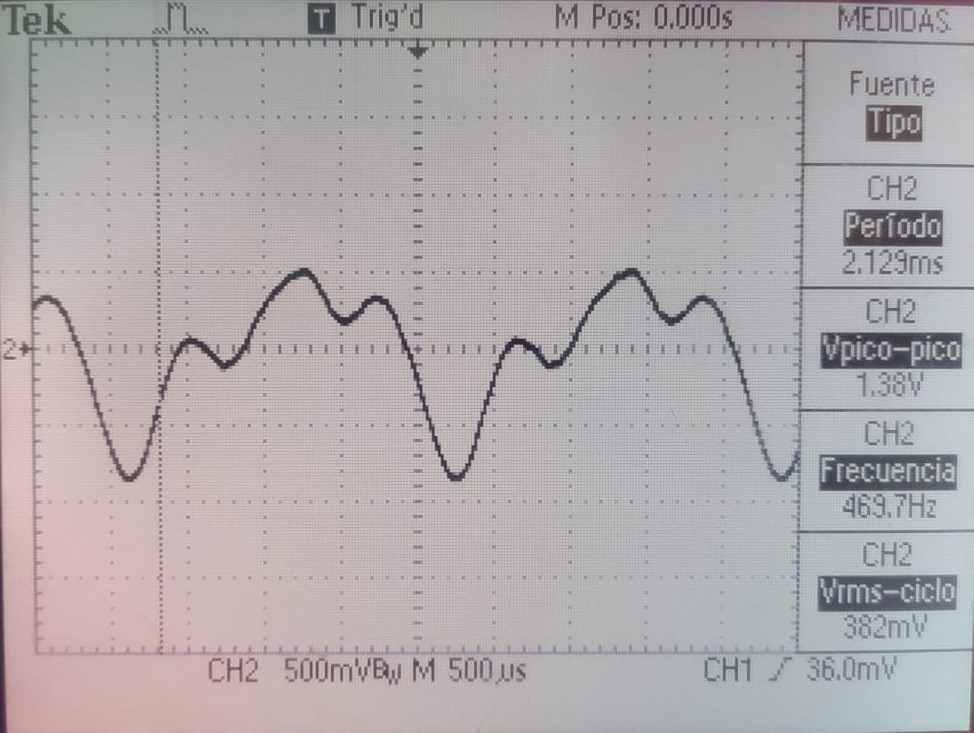
\includegraphics[width=10cm]{Osciloscopio.jpeg} 
\caption{Forma de Onda Producida por el DSP}
\end{figure}

Evidentemente no se puede mostrar en el documento el sonido que esta señal emitía, pero bajo el criterio de los integrantes del equipo y la evaluación del profesor, se puede asegurar que el tono generado si tiene similitud con el tono original por lo que se considera un resultado exitoso.

\section{Conclusiones}
El tono resultante, obtenido mediante este método si fue similar al adquirido. Si bien no fue tan fiel al original, si conserva una similitud general. 
\\
Consideramos que para conseguir una semejanza mas fiel al tono adquirido se tendría que incrementar la frecuencia de muestreo del tono adquirido. O mejor aún, del periodo elegido que posteriormente será replicado una y otra vez para generar el tono, se deben obtener más muestras, por decir algo, el doble de muestras de las que se consiguieron (94*2=188).
\\
Otra forma de mejorar la semejanza entre las señales seria la de tomar más periodos de la señal original para la sintetización de la señal, esto debido a que el sistema que produjo el sonido es un sistema mecánico y la amplitud asi como la forma de onda de salida de este varian según vibración de la caña de la boquilla que da origen al sonido, este comportamiento se puede observar en la figura 3 la cual si es comparada con la figura 8, solo reproduce la señal original un pequeño instante de tiempo

\section{Referencias}

  Proakis J $\&$ Manolakis D.(2007).Tratamiento Digital de Señales. 4a Edición.PEARSON Pretince Hall.
  \\\\
  Spectrum Digital Inc. (2003). TMS320C6713 DSK Technical Reference.
  \\\\

\section{Apéndice: Códigos.}
\subsection{Extracción de Muestras}
\lstinputlisting[language=Matlab]{audio_extract.m}
\subsection{Código DSP}
\lstinputlisting[language=C++]{sin1.cpp}
\end{document}
